\documentclass[UTF8]{article}
  \author {wide288}
  \title {Eclipse Manual}
\usepackage[colorlinks=true,linkcolor=blue,urlcolor=blue,citecolor=black]{hyperref}
\usepackage[UTF8]{ctex}
\usepackage{amsmath}
\usepackage{amssymb}
\usepackage{graphicx}
\begin{document}
  \maketitle
    \section{简介}
    Eclipse 使用手册
    此书是从 2017-11-2 有想法开始写的。因为在使用中感觉到 Eclipse 是我遇到过复杂度最高那类的软件。有必要写些系统性好的文章来记录下学习的过程。
    基于 Eclipse Oxygen R 版。
    \section{菜单介绍}
        \subsection{File}
            \begin{center} %图片居中
              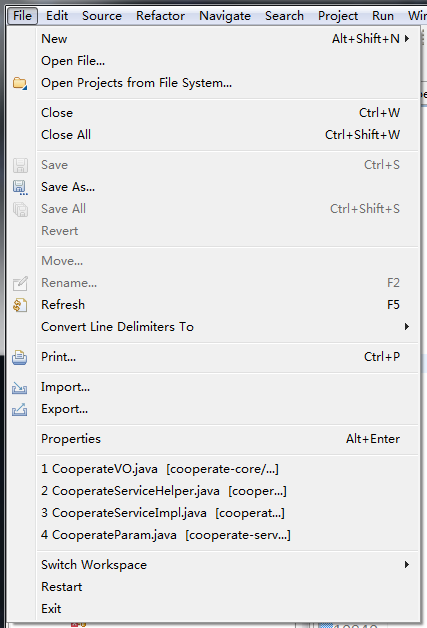
\includegraphics[width=200pt]{images/menu-file.png} %插入图片
            \end{center}
            \subsubsection{New}
              \paragraph{} 新建文件或项目
            \subsubsection{Open File...}
              \paragraph{} 打开文件
            \subsubsection{Open Projects form File System...}
              \paragraph{} 从文件系统打开项目
        \subsection{Edit}
            \begin{center} %图片居中
              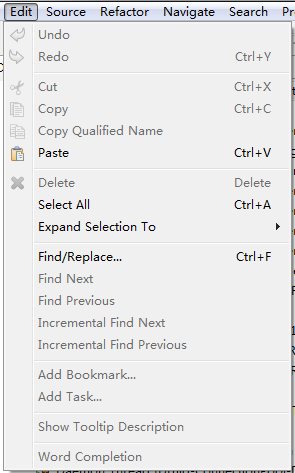
\includegraphics[width=200pt]{images/menu-edit.png} %插入图片
            \end{center}
            \paragraph{段落} 中文测试。
        \subsection{Source}
            \begin{center} %图片居中
              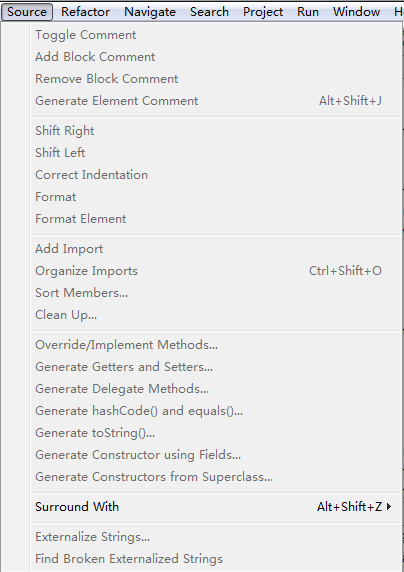
\includegraphics[width=200pt]{images/menu-source.png} %插入图片
            \end{center}

        \subsection{Refactor}
            \begin{center} %图片居中
              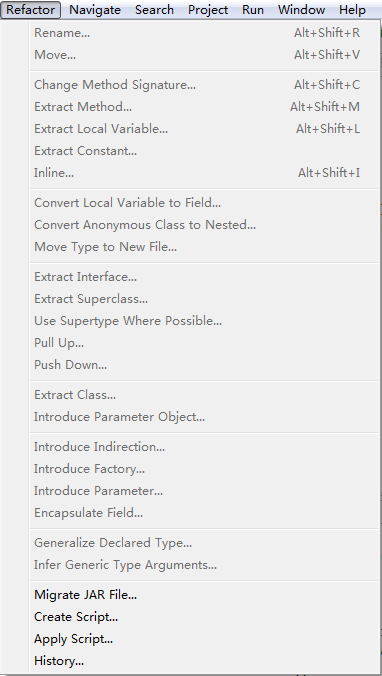
\includegraphics[width=200pt]{images/menu-refactor.png} %插入图片
            \end{center}
        \subsection{Navigate}
        \subsection{Search}
        \subsection{Project}
        \subsection{Run}
        \subsection{Window}
          \subsubsection{Preferences}
            \paragraph{Team} test3.
              \subparagraph{File Content} test4.
              \subparagraph{Git} test4.
    \section{Other}
    参考资料:
    eclipse 软件
    https://www.tutorialspoint.com/eclipse/eclipse_debug_configuration.htm
    http://help.eclipse.org/oxygen/index.jsp
    http://www.runoob.com/eclipse/eclipse-debugging-program.html (中文)
    论坛:http://www.eclipse.org/forums/index.php/f/89/
\end{document}
